%% main.tex — Relatório Final: SpaceX Reliability Study
%% Classe: abntex2

\documentclass[
    12pt,
    openright,
    oneside,
    a4paper,
    brazil
]{abntex2}

% ── Pacotes ────────────────────────────────────────────────────────────────
\usepackage[utf8]{inputenc}
\usepackage[T1]{fontenc}
\usepackage{lmodern}
\usepackage{graphicx}
\usepackage{booktabs}
\usepackage{multirow}
\usepackage{float}
\usepackage{amsmath}
\usepackage{hyperref}
\usepackage[brazilian,hyperpageref]{backref}
\usepackage[alf]{abntex2cite}

% ── Caminho das figuras ───────────────────────────────────────────────────
\graphicspath{{../graphs/}}

% ── Dados do documento ────────────────────────────────────────────────────
\titulo{Evidência Estatística de Confiabilidade em Sistemas de Foguetes Reutilizáveis: Um Estudo com Dados da SpaceX}
\autor{
    Lucas Gabriel Rocha Ferreira \and
    Gabriel Garcia\and
    Kaio Ribeiro\and
    Izac Regis\and
    Jônatas Pereira
}
\local{Brasil}
\data{Junho de 2026}
\orientador{Roberto Carlos Rodriguez}
\instituicao{Jala University}

\tipotrabalho{Relatório de Pesquisa}
\preambulo{Relatório final do estudo sobre a confiabilidade de sistemas de foguetes reutilizáveis, utilizando dados da SpaceX API v4, apresentado como requisito parcial para a disciplina de Estatística.}

% ── Configurações do PDF ──────────────────────────────────────────────────
\makeatletter
\hypersetup{
    pdftitle={\@title},
    pdfauthor={\@author},
    pdfsubject={\imprimirpreambulo},
    pdfkeywords={SpaceX}{reutilização}{confiabilidade}{estatística},
    colorlinks=true,
    linkcolor=blue,
    citecolor=blue,
    filecolor=magenta,
    urlcolor=blue,
    bookmarksdepth=4
}
\makeatother

% ══════════════════════════════════════════════════════════════════════════
\begin{document}

% ── Elementos pré-textuais ────────────────────────────────────────────────
\pretextual

% Capa
\imprimircapa

% Folha de rosto
\imprimirfolhaderosto

% ── Resumo ────────────────────────────────────────────────────────────────
\begin{resumo}
O presente trabalho analisa dados de lançamentos da SpaceX para verificar se a reutilização de propulsores orbitais tem impacto sobre a confiabilidade das missões. Foram utilizados 192 registros de boosters extraídos da SpaceX API v4, cobrindo o período de 2006 a 2022 e as famílias Falcon 1, Falcon 9 e Falcon Heavy. A análise foi conduzida com estatística descritiva, intervalos de confiança e tabulação cruzada com controle temporal. Os boosters reutilizados apresentaram 100\% de sucesso (149 de 149), contra 88,37\% dos virgens (38 de 43), e não foi observada degradação mesmo em boosters com até 13 voos acumulados. No entanto, a presença de viés temporal e viés de seleção nos dados impede afirmações definitivas de causalidade. De modo geral, os resultados sugerem que a reutilização não compromete a confiabilidade das missões.

\vspace{\onelineskip}
\noindent
\textbf{Palavras-chave}: SpaceX. Reutilização de foguetes. Confiabilidade. Análise estatística.
\end{resumo}

% ── Sumário ───────────────────────────────────────────────────────────────
\pdfbookmark[0]{\contentsname}{toc}
\tableofcontents*
\cleardoublepage

% ── Elementos textuais ────────────────────────────────────────────────────
\textual

%% sections/introduction.tex

\chapter{Introdução}

Nos últimos anos, a indústria aeroespacial passou por mudanças consideráveis com a entrada de empresas privadas no mercado de lançamentos orbitais. A SpaceX, fundada em 2002 por Elon Musk, foi uma das principais responsáveis por essa transformação ao apostar em algo que até então era considerado inviável: pousar e reutilizar os propulsores de primeiro estágio dos seus foguetes \cite{jones2018spacex_reuse}.

Antes disso, o padrão da indústria era descartar o foguete inteiro após cada lançamento. Cada missão exigia a construção de um veículo novo, o que tornava o acesso ao espaço extremamente caro. A SpaceX começou a mudar isso em 2015, quando conseguiu pousar com sucesso o primeiro estágio de um Falcon 9, e desde então vem reutilizando seus boosters com frequência cada vez maior \cite{zapata2017spacex_economics}.

Essa estratégia de reutilização traz benefícios econômicos claros, mas levanta uma dúvida legítima do ponto de vista de engenharia: será que usar o mesmo propulsor várias vezes não compromete a segurança e a confiabilidade das missões? Se boosters reutilizados falhassem mais, a economia obtida com a reutilização poderia não compensar o risco.

\section{Pergunta de Pesquisa}

É exatamente essa a pergunta que este trabalho busca responder:

\begin{quote}
\textit{A reutilização de foguetes afeta a confiabilidade das missões?}
\end{quote}

\section{Hipótese}

Nossa hipótese é que boosters reutilizados mantêm — ou até melhoram — a confiabilidade ao longo de múltiplos lançamentos, o que indicaria que a reutilização é uma estratégia viável sem comprometer o sucesso das missões.

\section{Objetivos}

\subsection{Objetivo Geral}

Analisar dados históricos de lançamentos da SpaceX para avaliar se a reutilização de propulsores tem algum impacto sobre a confiabilidade das missões.

\subsection{Objetivos Específicos}

\begin{enumerate}
    \item Mapear como a taxa de sucesso dos lançamentos evoluiu entre 2006 e 2022;
    \item Comparar o desempenho de boosters virgens com o de boosters que já haviam voado antes;
    \item Verificar se existe degradação à medida que um booster acumula mais voos (análise dose-resposta);
    \item Comparar a confiabilidade das diferentes famílias de foguetes da SpaceX (Falcon 1, Falcon 9, Falcon Heavy).
\end{enumerate}

\section{Estrutura do Trabalho}

O restante deste relatório está organizado da seguinte forma: o \autoref{chap:methodology} apresenta de onde vieram os dados, como foram tratados e quais métodos estatísticos foram usados; o \autoref{chap:results} traz os resultados de cada análise; o \autoref{chap:discussion} discute o que esses resultados significam quando olhados em conjunto, apontando também suas limitações; e o \autoref{chap:conclusion} fecha com as conclusões e sugestões para trabalhos futuros.

%% sections/methodology.tex

\chapter{Metodologia}
\label{chap:methodology}

Neste capítulo, descrevemos a origem dos dados, como foram coletados e tratados, a estrutura do dataset final e os métodos estatísticos que utilizamos.

\section{Fonte de Dados}

Os dados utilizados neste estudo foram obtidos da \textbf{SpaceX API v4} \cite{spacex_api}, uma API REST de código aberto mantida pela comunidade que reúne informações sobre os lançamentos, foguetes e propulsores da SpaceX. Utilizamos três endpoints:

\begin{itemize}
    \item \texttt{/launches} — dados de cada missão (data, nome, resultado, identificadores de foguete e propulsor);
    \item \texttt{/rockets} — informações sobre as famílias de foguetes (Falcon 1, Falcon 9, Falcon Heavy);
    \item \texttt{/cores} — histórico individual de cada propulsor (quantas vezes voou, status atual).
\end{itemize}

A API não exige autenticação e sua estrutura de dados foi validada antes do início da coleta \cite{spacex_api_docs}.

\section{Coleta e Tratamento dos Dados (ETL)}

Todo o processo de coleta e tratamento foi implementado em Python 3 \cite{python} com a biblioteca Pandas \cite{mckinney2010pandas}, e está documentado no notebook \texttt{lucas\_data\_extraction.ipynb}. As etapas foram as seguintes:

\begin{enumerate}
    \item \textbf{Extração}: Coletamos 205 lançamentos do endpoint \texttt{/launches} e cruzamos com os dados de \texttt{/rockets} e \texttt{/cores} usando os identificadores de cada registro;
    \item \textbf{Transformação}: Calculamos campos derivados como \texttt{launch\_year} (extraído da data) e \texttt{is\_reused} (se o booster já tinha voado antes). Também tratamos as missões do Falcon Heavy, que usa 3 boosters e gera 3 linhas por lançamento. Durante essa etapa, corrigimos um bug no cálculo do \texttt{reuse\_count} que estava usando o tamanho de uma lista em vez do valor direto da API;
    \item \textbf{Limpeza}: Removemos 23 registros que tinham o campo \texttt{success} nulo — eram missões que estavam planejadas para 2022 mas ainda não tinham sido executadas no momento da coleta;
    \item \textbf{Validação}: Verificamos que o dataset final tinha as 9 colunas esperadas, nenhum valor nulo, nenhuma duplicata, e que os tipos de dados estavam corretos.
\end{enumerate}

\section{Dataset Final}

Após o tratamento, chegamos ao dataset descrito na \autoref{tab:dataset_overview}.

\begin{table}[H]
\centering
\caption{Características do dataset final (\texttt{processed\_dataset\_v1.csv}).}
\label{tab:dataset_overview}
\begin{tabular}{ll}
\toprule
\textbf{Aspecto}              & \textbf{Valor} \\
\midrule
Registros                      & 192 \\
Variáveis                     & 9 \\
Valores nulos                  & 0 \\
Duplicatas                     & 0 \\
Período                        & 2006--2022 \\
Unidade de observação          & Booster (propulsor) por missão \\
Taxa de sucesso global         & 97,40\% \\
\bottomrule
\end{tabular}
\end{table}

Um ponto que vale destacar: a unidade de observação do dataset é o \textbf{booster}, não o lançamento. Essa decisão foi intencional — como a pergunta de pesquisa trata da confiabilidade do \textit{propulsor}, faz sentido que cada booster seja analisado individualmente. Na prática, isso significa que um lançamento do Falcon Heavy (que usa 3 boosters) gera 3 linhas no dataset, cada uma com seu próprio \texttt{reuse\_count}.

A \autoref{tab:data_dictionary} descreve as variáveis disponíveis.

\begin{table}[H]
\centering
\caption{Dicionário de dados.}
\label{tab:data_dictionary}
\begin{tabular}{llp{7cm}}
\toprule
\textbf{Variável} & \textbf{Tipo} & \textbf{Descrição} \\
\midrule
\texttt{launch\_year}   & int64   & Ano do lançamento (2006--2022) \\
\texttt{launch\_name}   & string  & Nome oficial da missão \\
\texttt{flight\_number} & int64   & Número sequencial do voo \\
\texttt{success}        & bool    & Resultado da missão (True/False) \\
\texttt{rocket\_name}   & string  & Família do foguete (Falcon 1, 9, Heavy) \\
\texttt{core\_id}       & string  & Identificador único do booster \\
\texttt{reuse\_count}   & int64   & Nº de voos anteriores do booster (0--13) \\
\texttt{is\_reused}     & bool    & Se o booster já havia voado (reuse\_count $> 0$) \\
\texttt{launch\_date}   & string  & Data e hora em UTC (formato ISO 8601) \\
\bottomrule
\end{tabular}
\end{table}

\section{Métodos Estatísticos}

Cada membro da equipe ficou responsável por uma dimensão da análise, mas todos utilizaram um conjunto comum de métodos:

\begin{itemize}
    \item \textbf{Estatística descritiva}: frequências, proporções e taxas de sucesso para cada grupo analisado;
    \item \textbf{Intervalos de confiança}: IC de 95\% para as taxas de sucesso anuais, o que ajuda a avaliar a incerteza das estimativas, especialmente nos anos com poucos lançamentos;
    \item \textbf{Tabulação cruzada}: comparação de taxas entre grupos (virgens vs.\ reutilizados; entre famílias de foguetes; entre faixas de experiência);
    \item \textbf{Análise dose-resposta}: avaliação de como a taxa de sucesso se comporta à medida que o \texttt{reuse\_count} aumenta, para verificar se existe efeito de desgaste;
    \item \textbf{Controle temporal}: estratificação por ano para tentar separar o efeito da reutilização do efeito da maturidade operacional da empresa.
\end{itemize}

\section{Ferramentas}

As análises foram feitas em Python 3 usando Pandas \cite{mckinney2010pandas} para manipulação de dados, Matplotlib \cite{hunter2007matplotlib} para os gráficos, e SciPy \cite{virtanen2020scipy} para os testes estatísticos. Todo o código está versionado no GitHub.

%% sections/results.tex

\chapter{Resultados}
\label{chap:results}

Neste capítulo, apresentamos os resultados das quatro análises conduzidas pela equipe. Cada seção aborda uma dimensão diferente da pergunta de pesquisa.

% ══════════════════════════════════════════════════════════════════════════
\section{Tendências Temporais}
\label{sec:temporal}

A análise temporal, conduzida por Gabriel, buscou entender como a confiabilidade dos lançamentos da SpaceX mudou ao longo do período de 2006 a 2022.

\subsection{Evolução da Taxa de Sucesso}

A trajetória da taxa de sucesso ao longo dos anos pode ser vista na \autoref{fig:gabriel_success}. Nos anos iniciais (2006--2008), quando a SpaceX ainda operava o Falcon 1, os resultados eram instáveis — a taxa de sucesso variou entre 0\% e 50\%. A partir de 2010, com a entrada do Falcon 9, o cenário mudou bastante: a taxa subiu para 100\% e permaneceu acima de 85\% em todos os anos seguintes. De 2017 em diante, todos os lançamentos foram bem-sucedidos.

\begin{figure}[H]
    \centering
    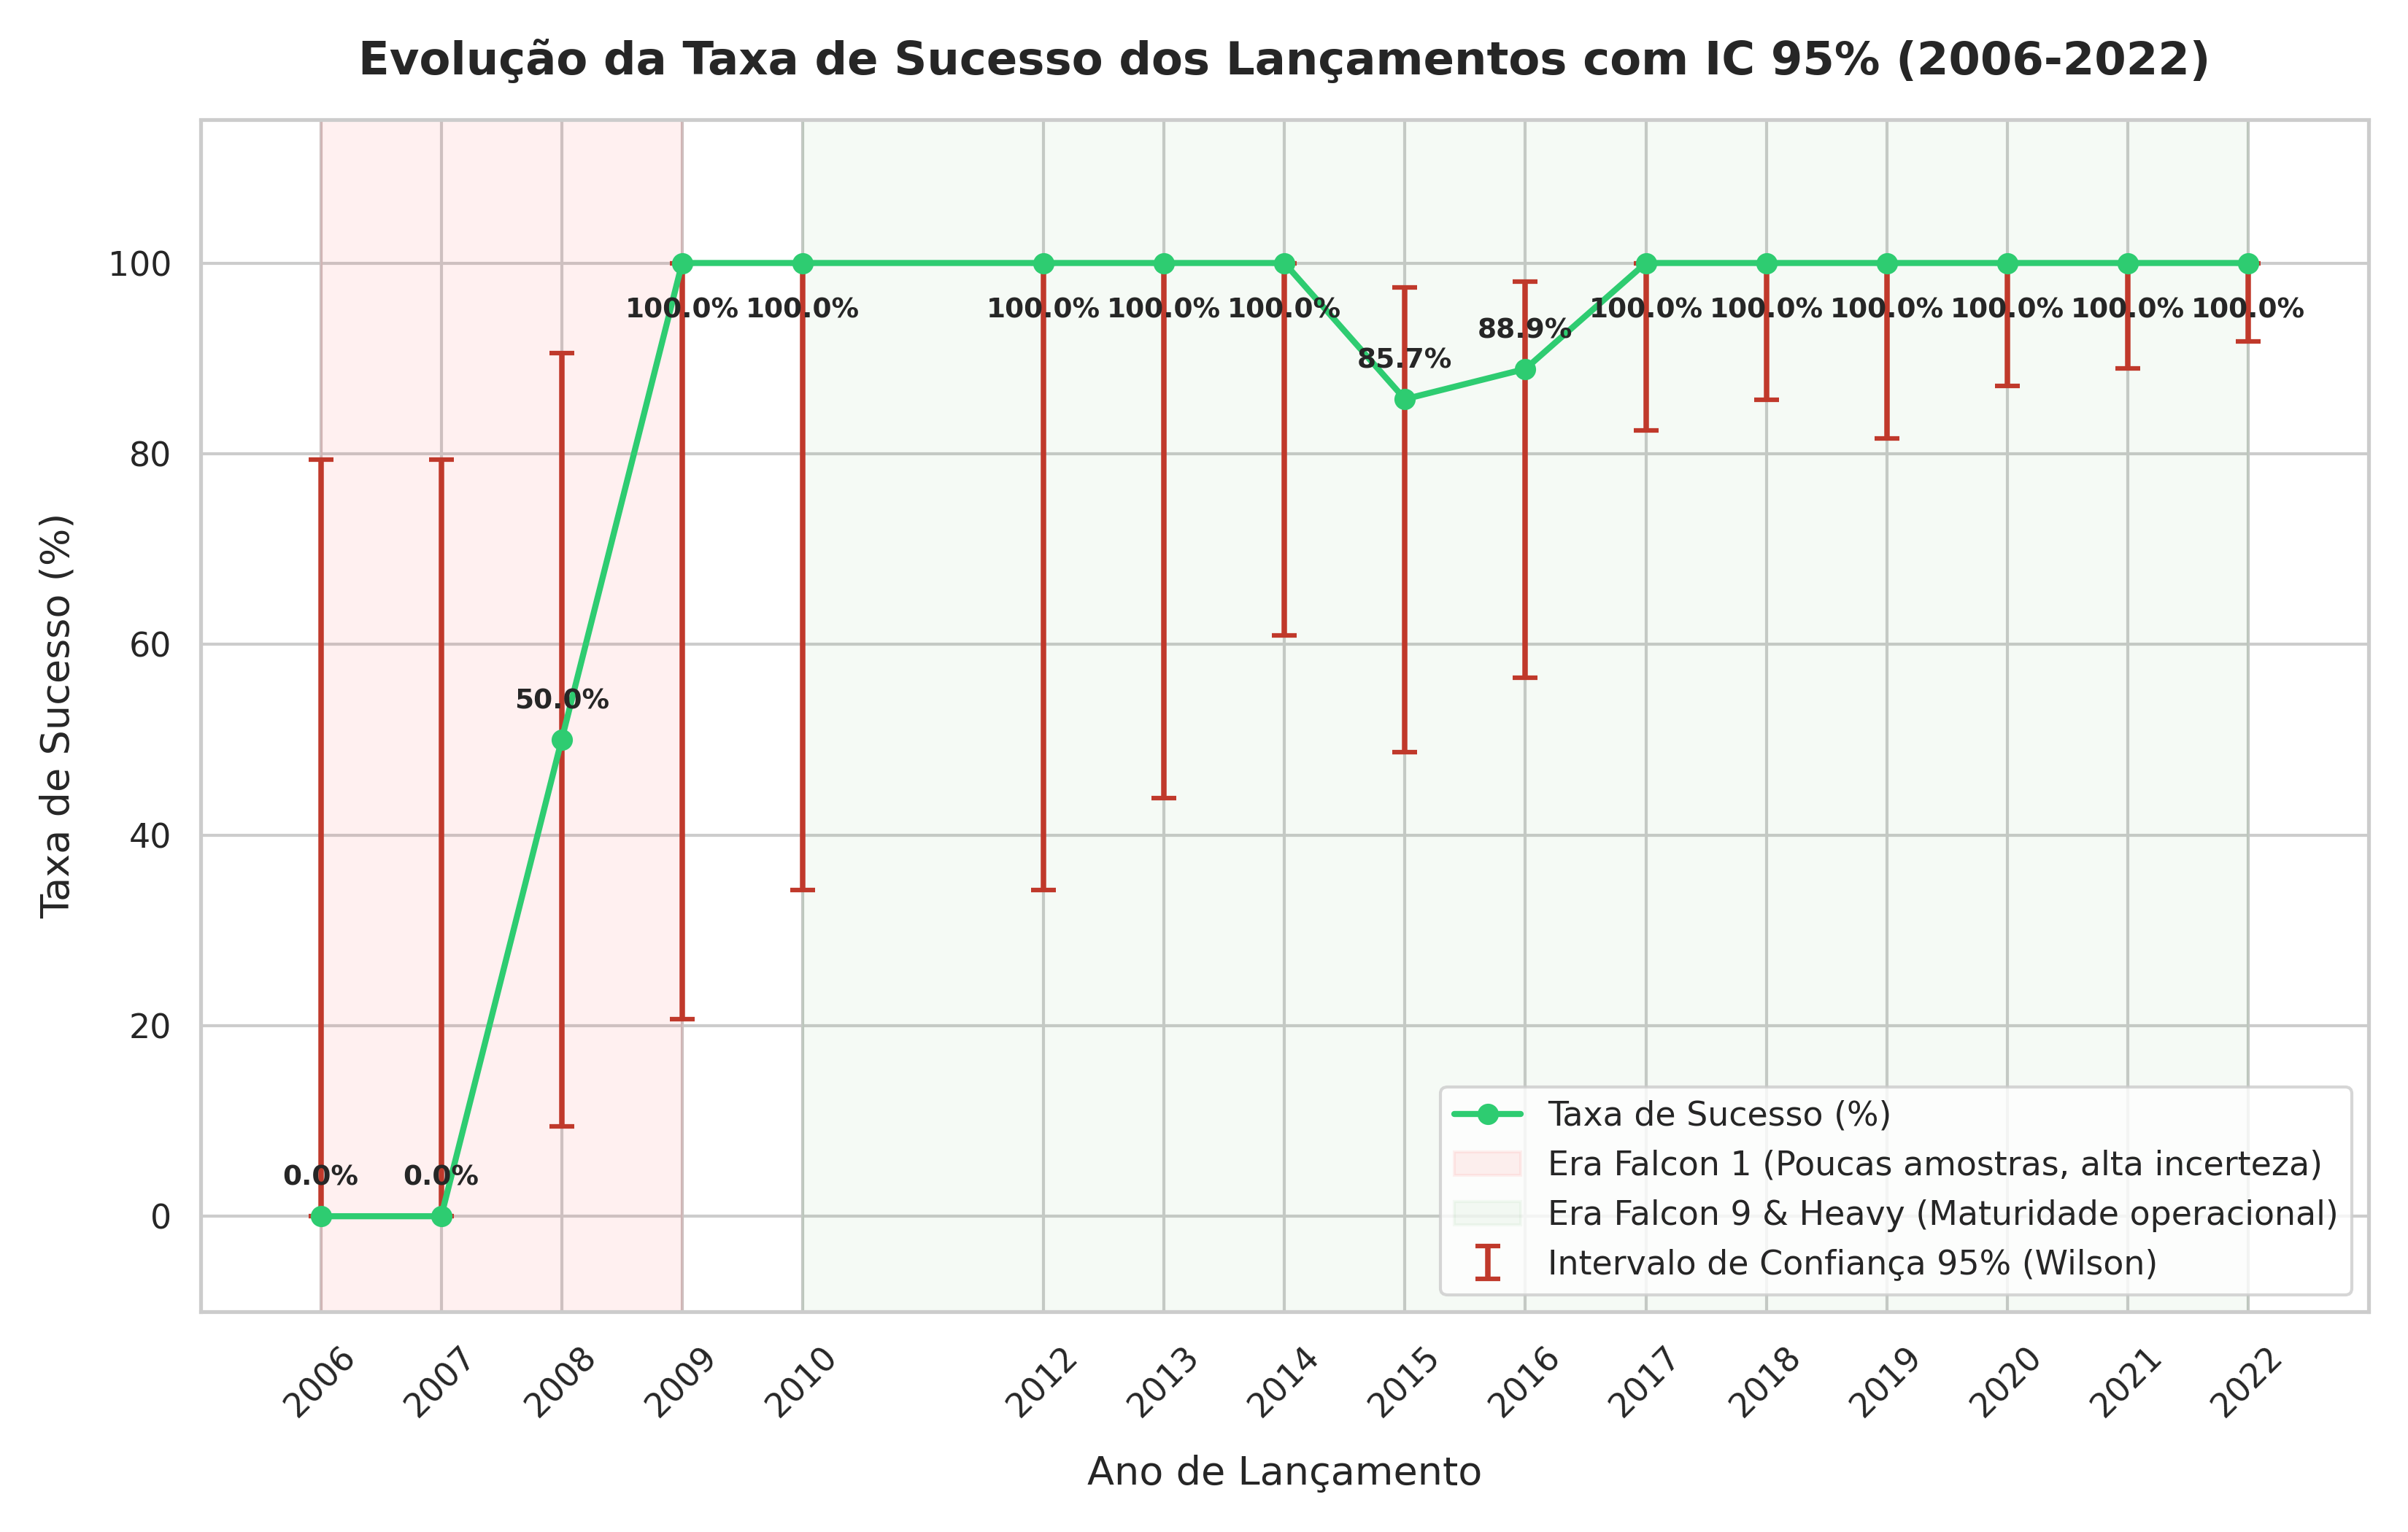
\includegraphics[width=0.85\textwidth]{gabriel_success_rate_per_year.png}
    \caption{Taxa de sucesso dos lançamentos da SpaceX por ano (2006--2022), com intervalos de confiança de 95\%.}
    \label{fig:gabriel_success}
\end{figure}

\subsection{Crescimento Operacional}

Outro aspecto relevante é o volume de lançamentos. A SpaceX saiu de 1--2 lançamentos por ano entre 2006 e 2010 para 43 lançamentos em 2022 (\autoref{fig:gabriel_launches}). O que chama atenção é que esse aumento de escala não veio acompanhado de perda de qualidade — a confiabilidade se manteve alta durante todo o período de crescimento.

\begin{figure}[H]
    \centering
    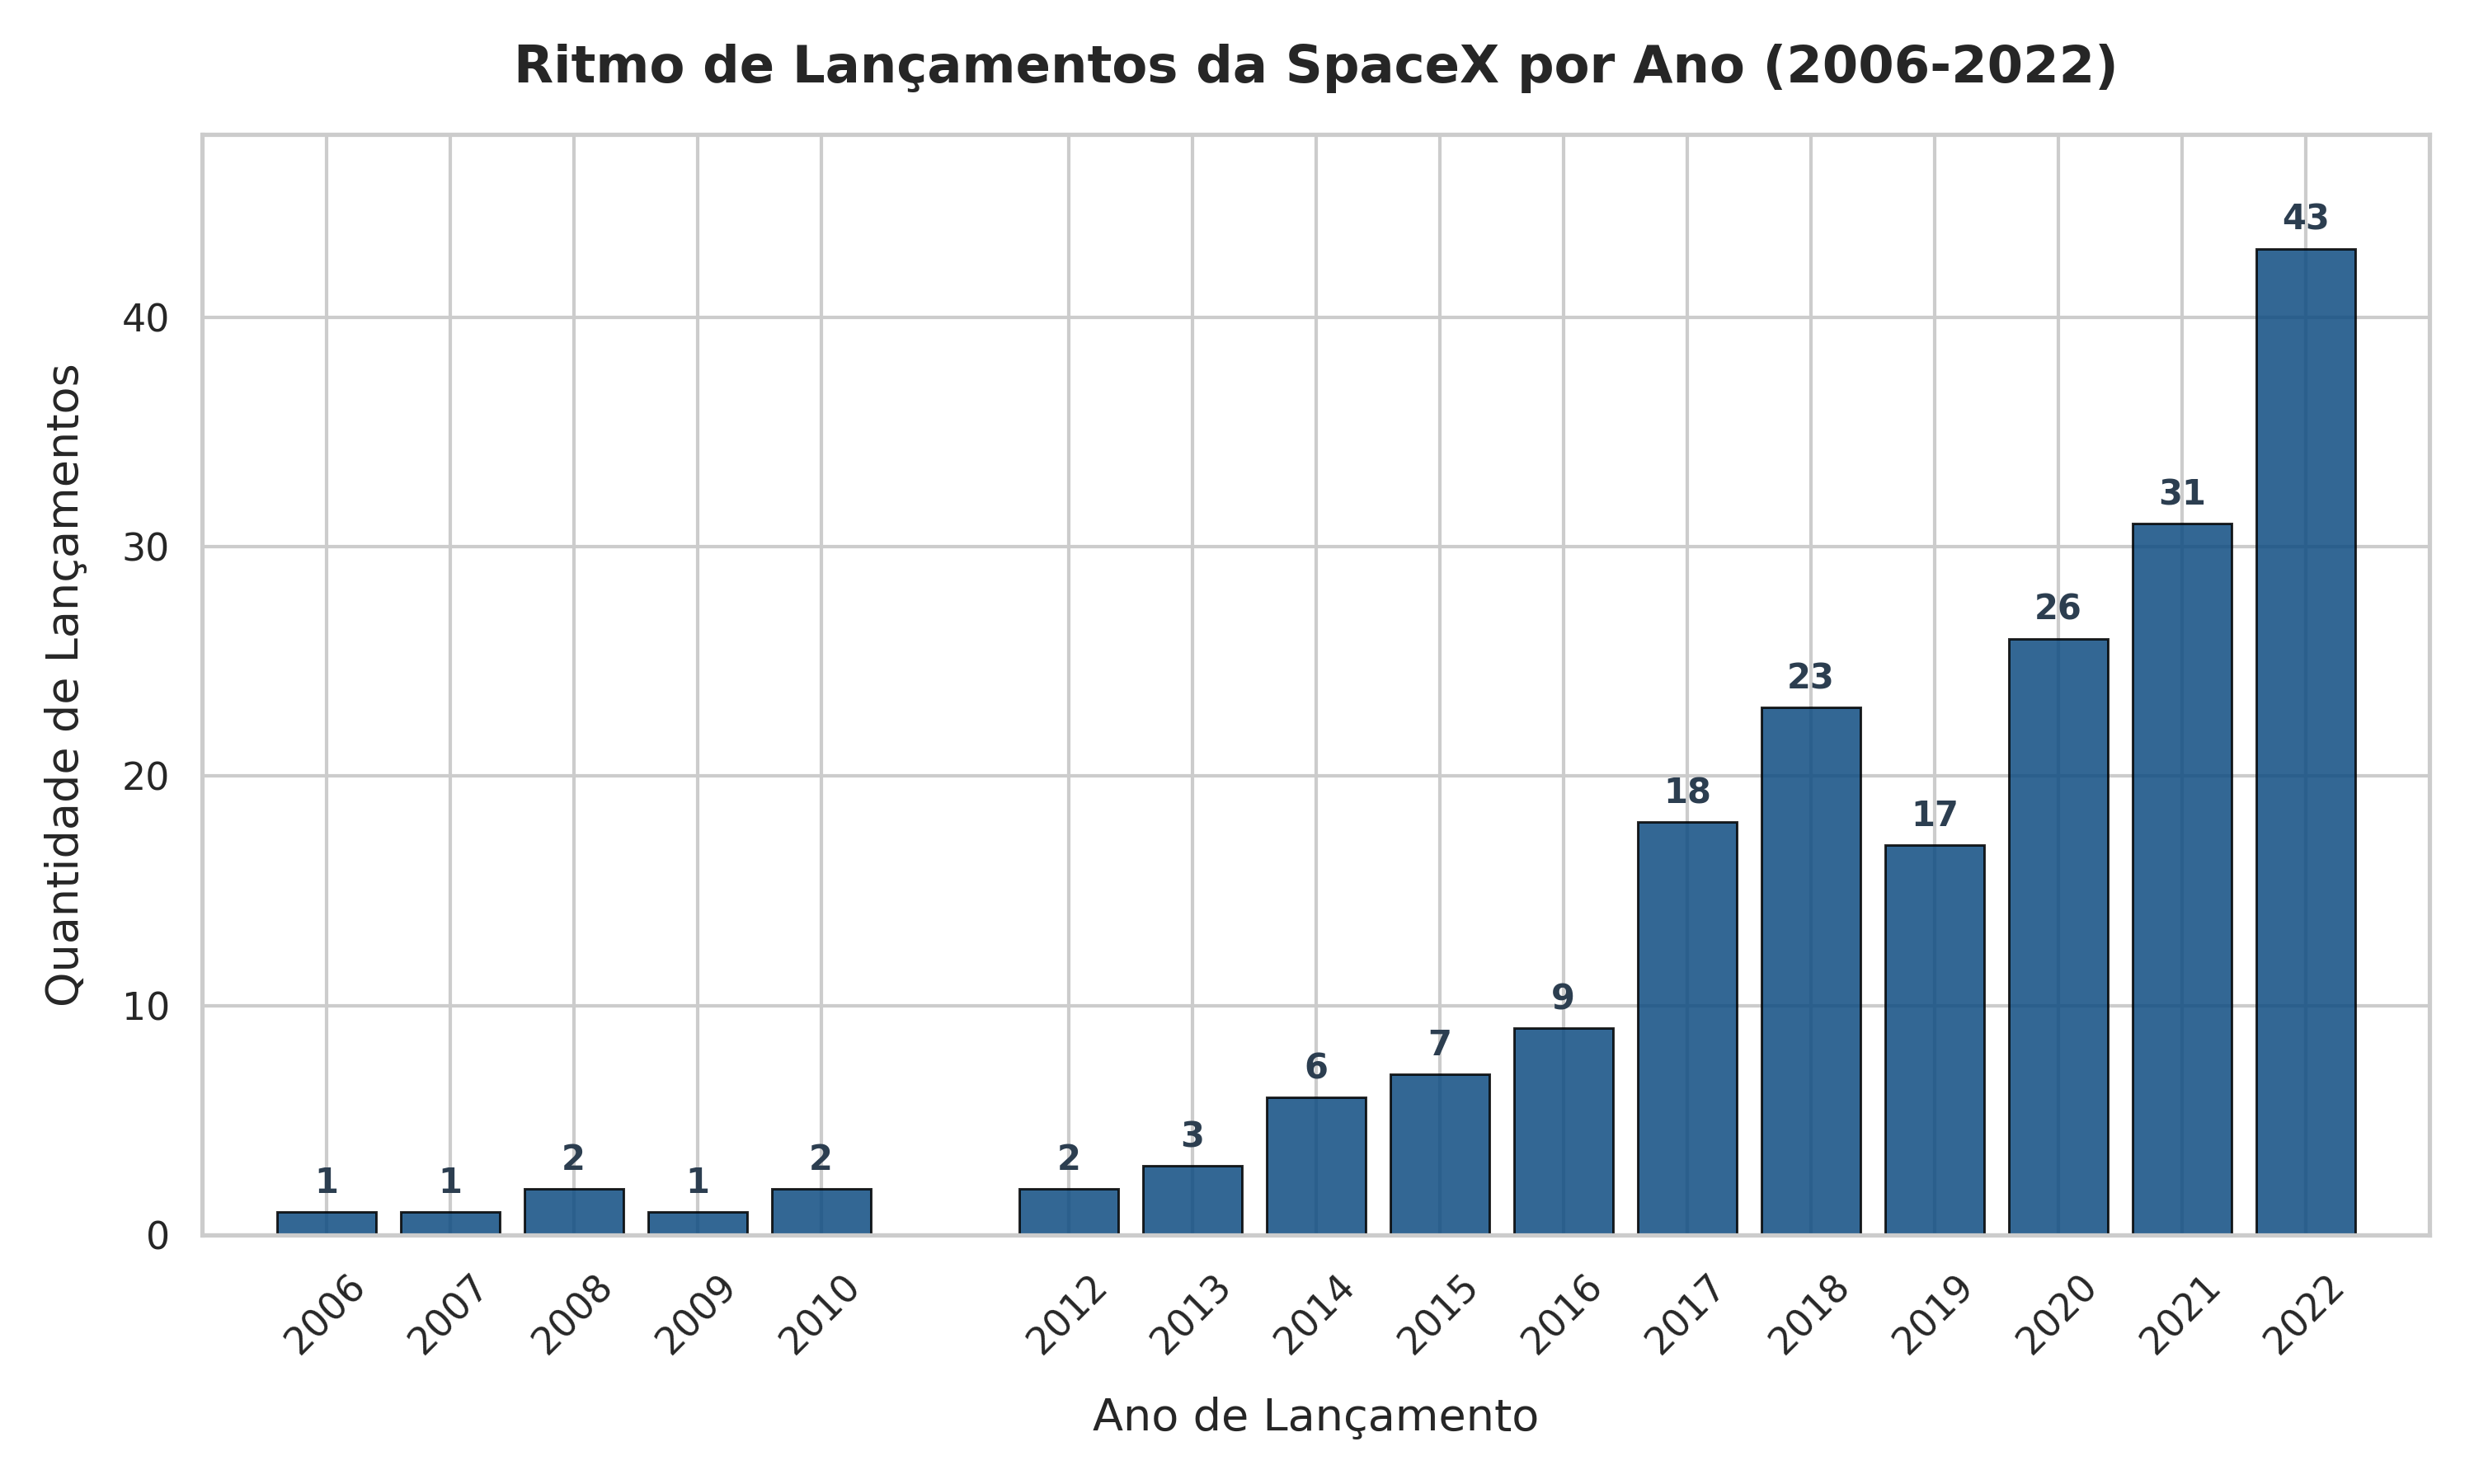
\includegraphics[width=0.85\textwidth]{gabriel_launches_per_year.png}
    \caption{Número de lançamentos da SpaceX por ano (2006--2022).}
    \label{fig:gabriel_launches}
\end{figure}

\subsection{Adoção da Reutilização}

A prática de reutilizar boosters foi se consolidando ao longo do tempo. Antes de 2016, nenhum booster havia sido reutilizado. Em 2020, praticamente 100\% dos boosters utilizados já tinham voos anteriores (\autoref{fig:gabriel_reuse}). Esse crescimento acompanhou o período de maior confiabilidade da empresa.

\begin{figure}[H]
    \centering
    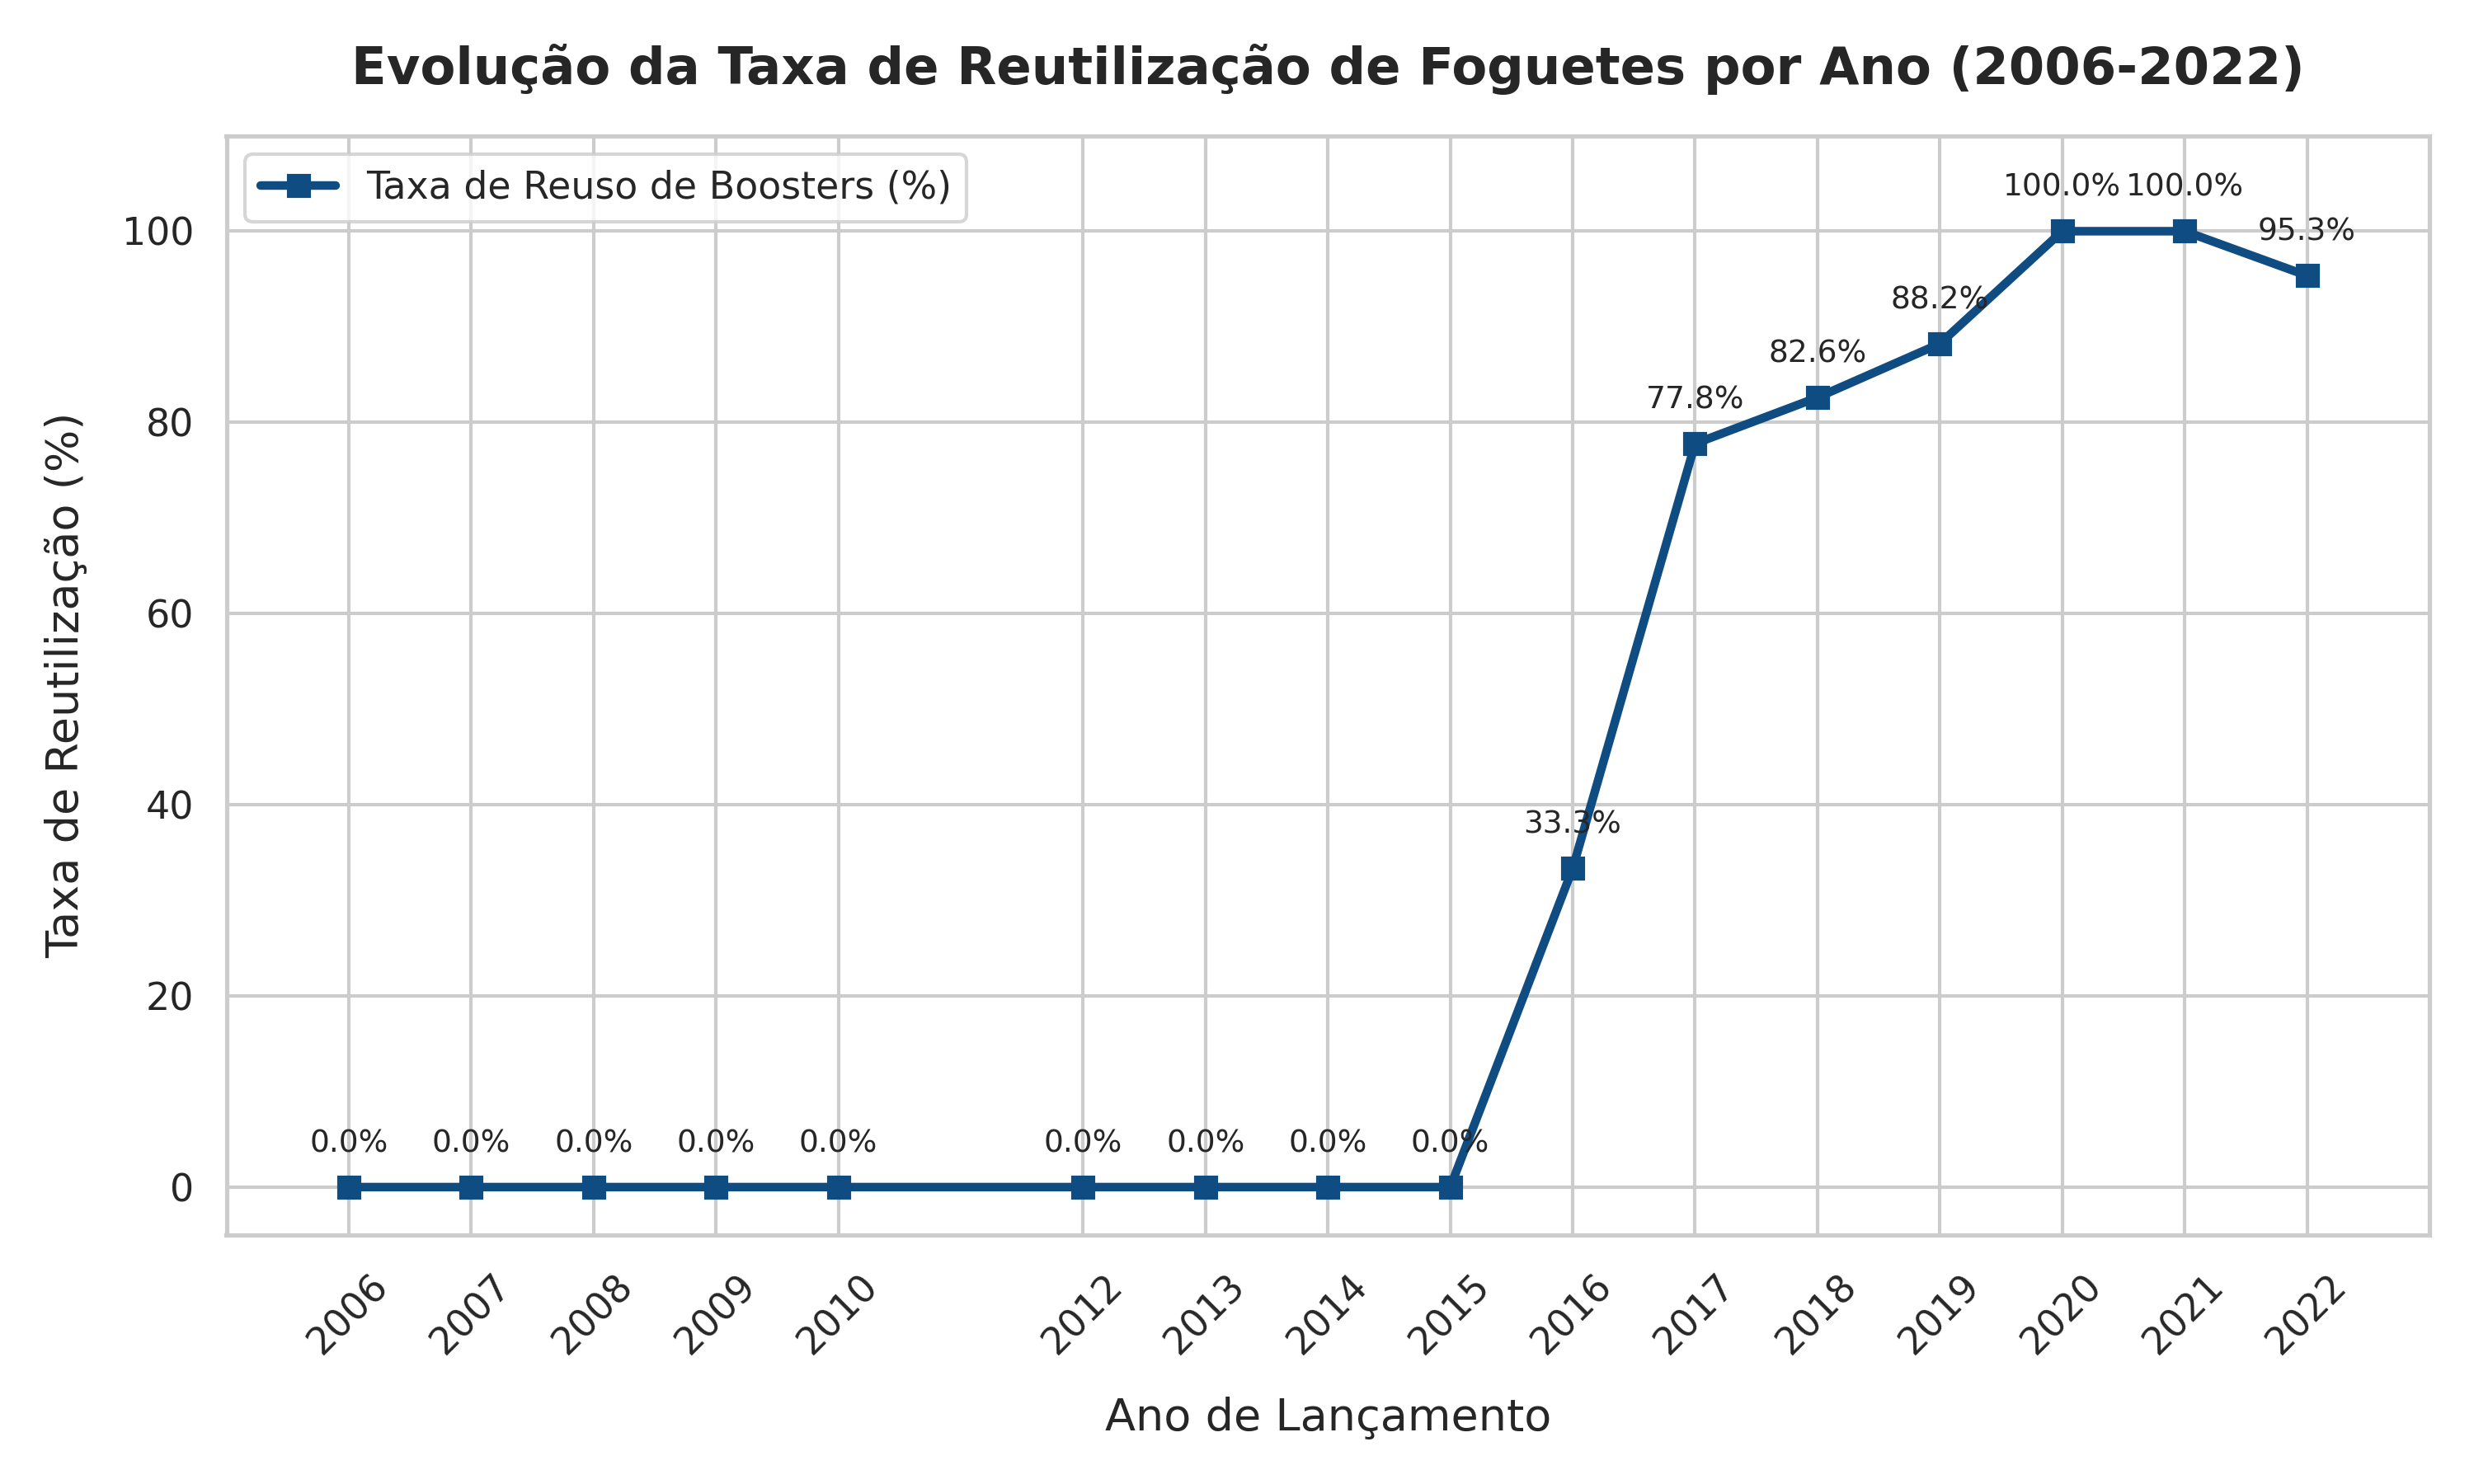
\includegraphics[width=0.85\textwidth]{gabriel_reuse_rate_per_year.png}
    \caption{Taxa de reutilização de boosters por ano.}
    \label{fig:gabriel_reuse}
\end{figure}

% ══════════════════════════════════════════════════════════════════════════
\section{Impacto da Reutilização}
\label{sec:reusability}

Kaio foi direto na pergunta central do projeto: será que reutilizar um booster compromete o resultado da missão? Para responder, ele separou os registros em dois grupos — virgens e reutilizados — e comparou os resultados.

\subsection{Comparação Global}

Os números estão na \autoref{tab:kaio_stats}. Dos 149 voos com boosters reutilizados, nenhum falhou. Já entre os 43 voos com boosters virgens, 5 resultaram em falha, o que dá uma taxa de 88,37\%. A diferença entre os dois grupos é de 11,63 pontos percentuais.

\begin{table}[H]
\centering
\caption{Taxas de sucesso comparadas entre boosters virgens e reutilizados.}
\label{tab:kaio_stats}
\begin{tabular}{lrrr}
\toprule
\textbf{Tipo} & \textbf{Quantidade} & \textbf{Sucessos} & \textbf{Taxa de Sucesso} \\
\midrule
Virgem       & 43  & 38  & 88,37\% \\
Reutilizado  & 149 & 149 & 100,00\% \\
\midrule
\textbf{Total} & \textbf{192} & \textbf{187} & \textbf{97,40\%} \\
\bottomrule
\end{tabular}
\end{table}

\begin{figure}[H]
    \centering
    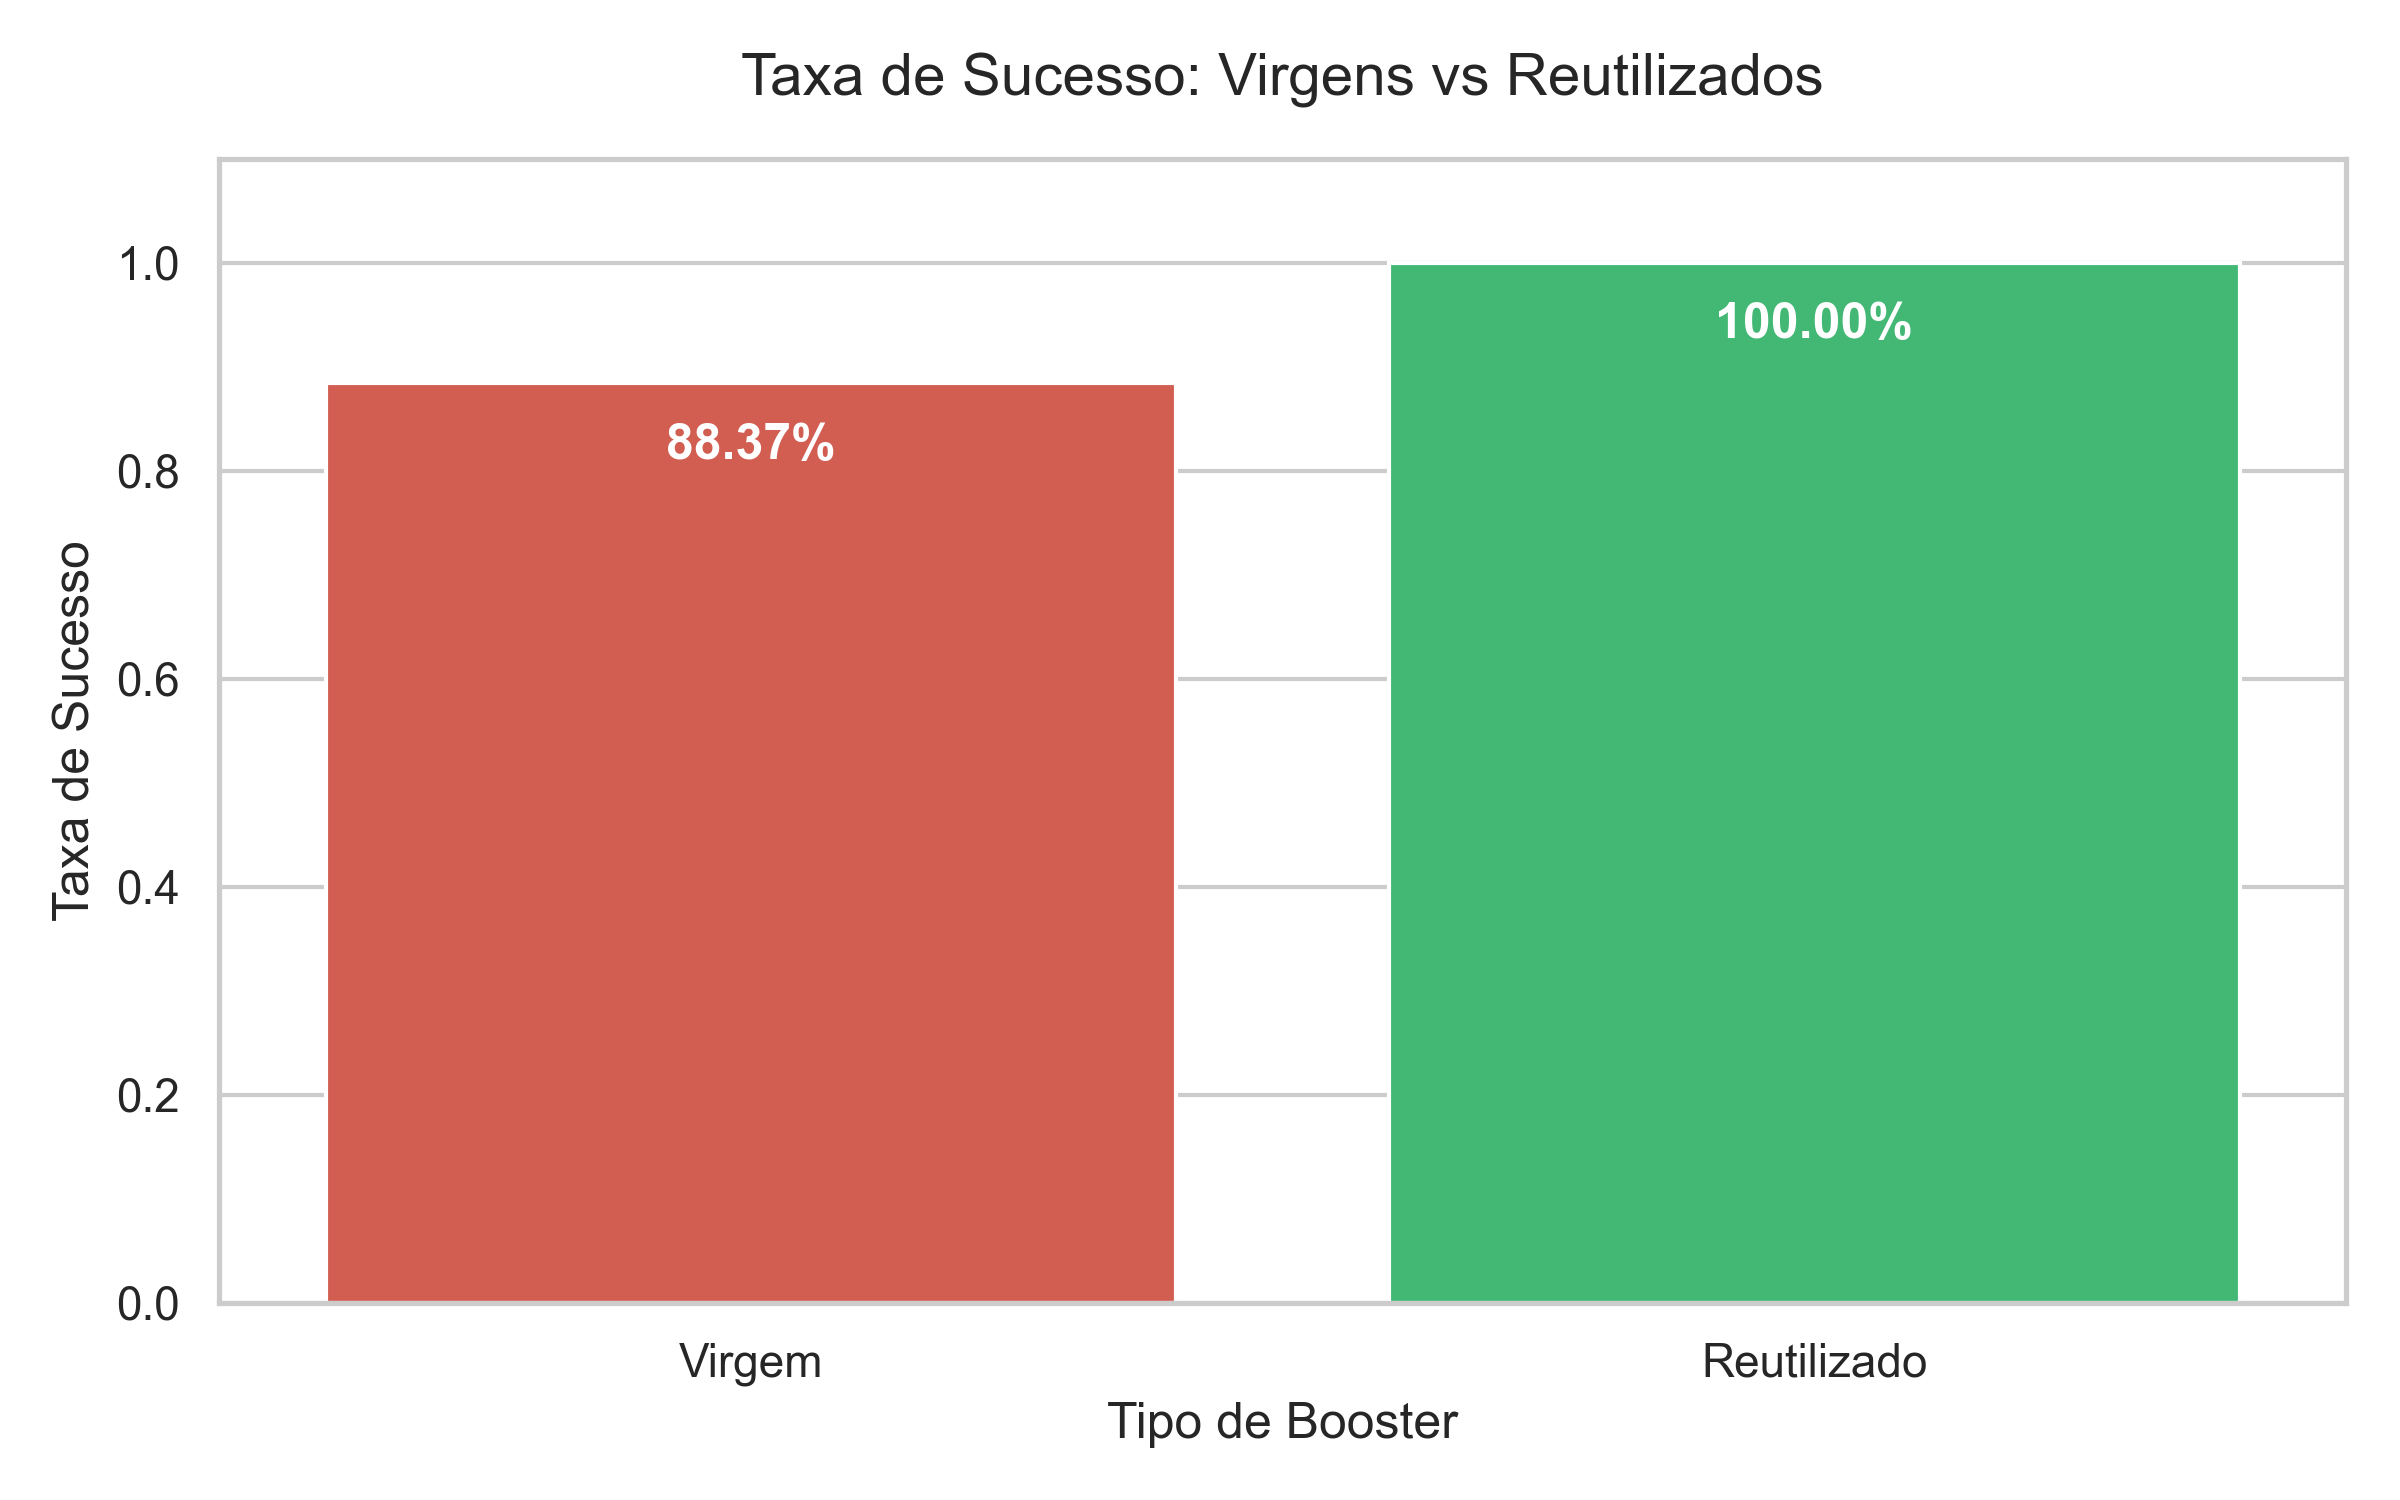
\includegraphics[width=0.85\textwidth]{kaio_overall_success_rate.png}
    \caption{Comparação visual das taxas de sucesso: virgens vs.\ reutilizados.}
    \label{fig:kaio_overall}
\end{figure}

\subsection{Controle Temporal}

Para verificar se essa diferença não era apenas um reflexo da época, o Kaio estratificou os dados por ano (\autoref{fig:kaio_temporal}). O que se observou é que as falhas dos boosters virgens se concentram nos primeiros anos do programa (2006--2015). A partir de 2016, quando os reutilizados começam a aparecer, ambos os grupos apresentam taxas de sucesso altas.

\begin{figure}[H]
    \centering
    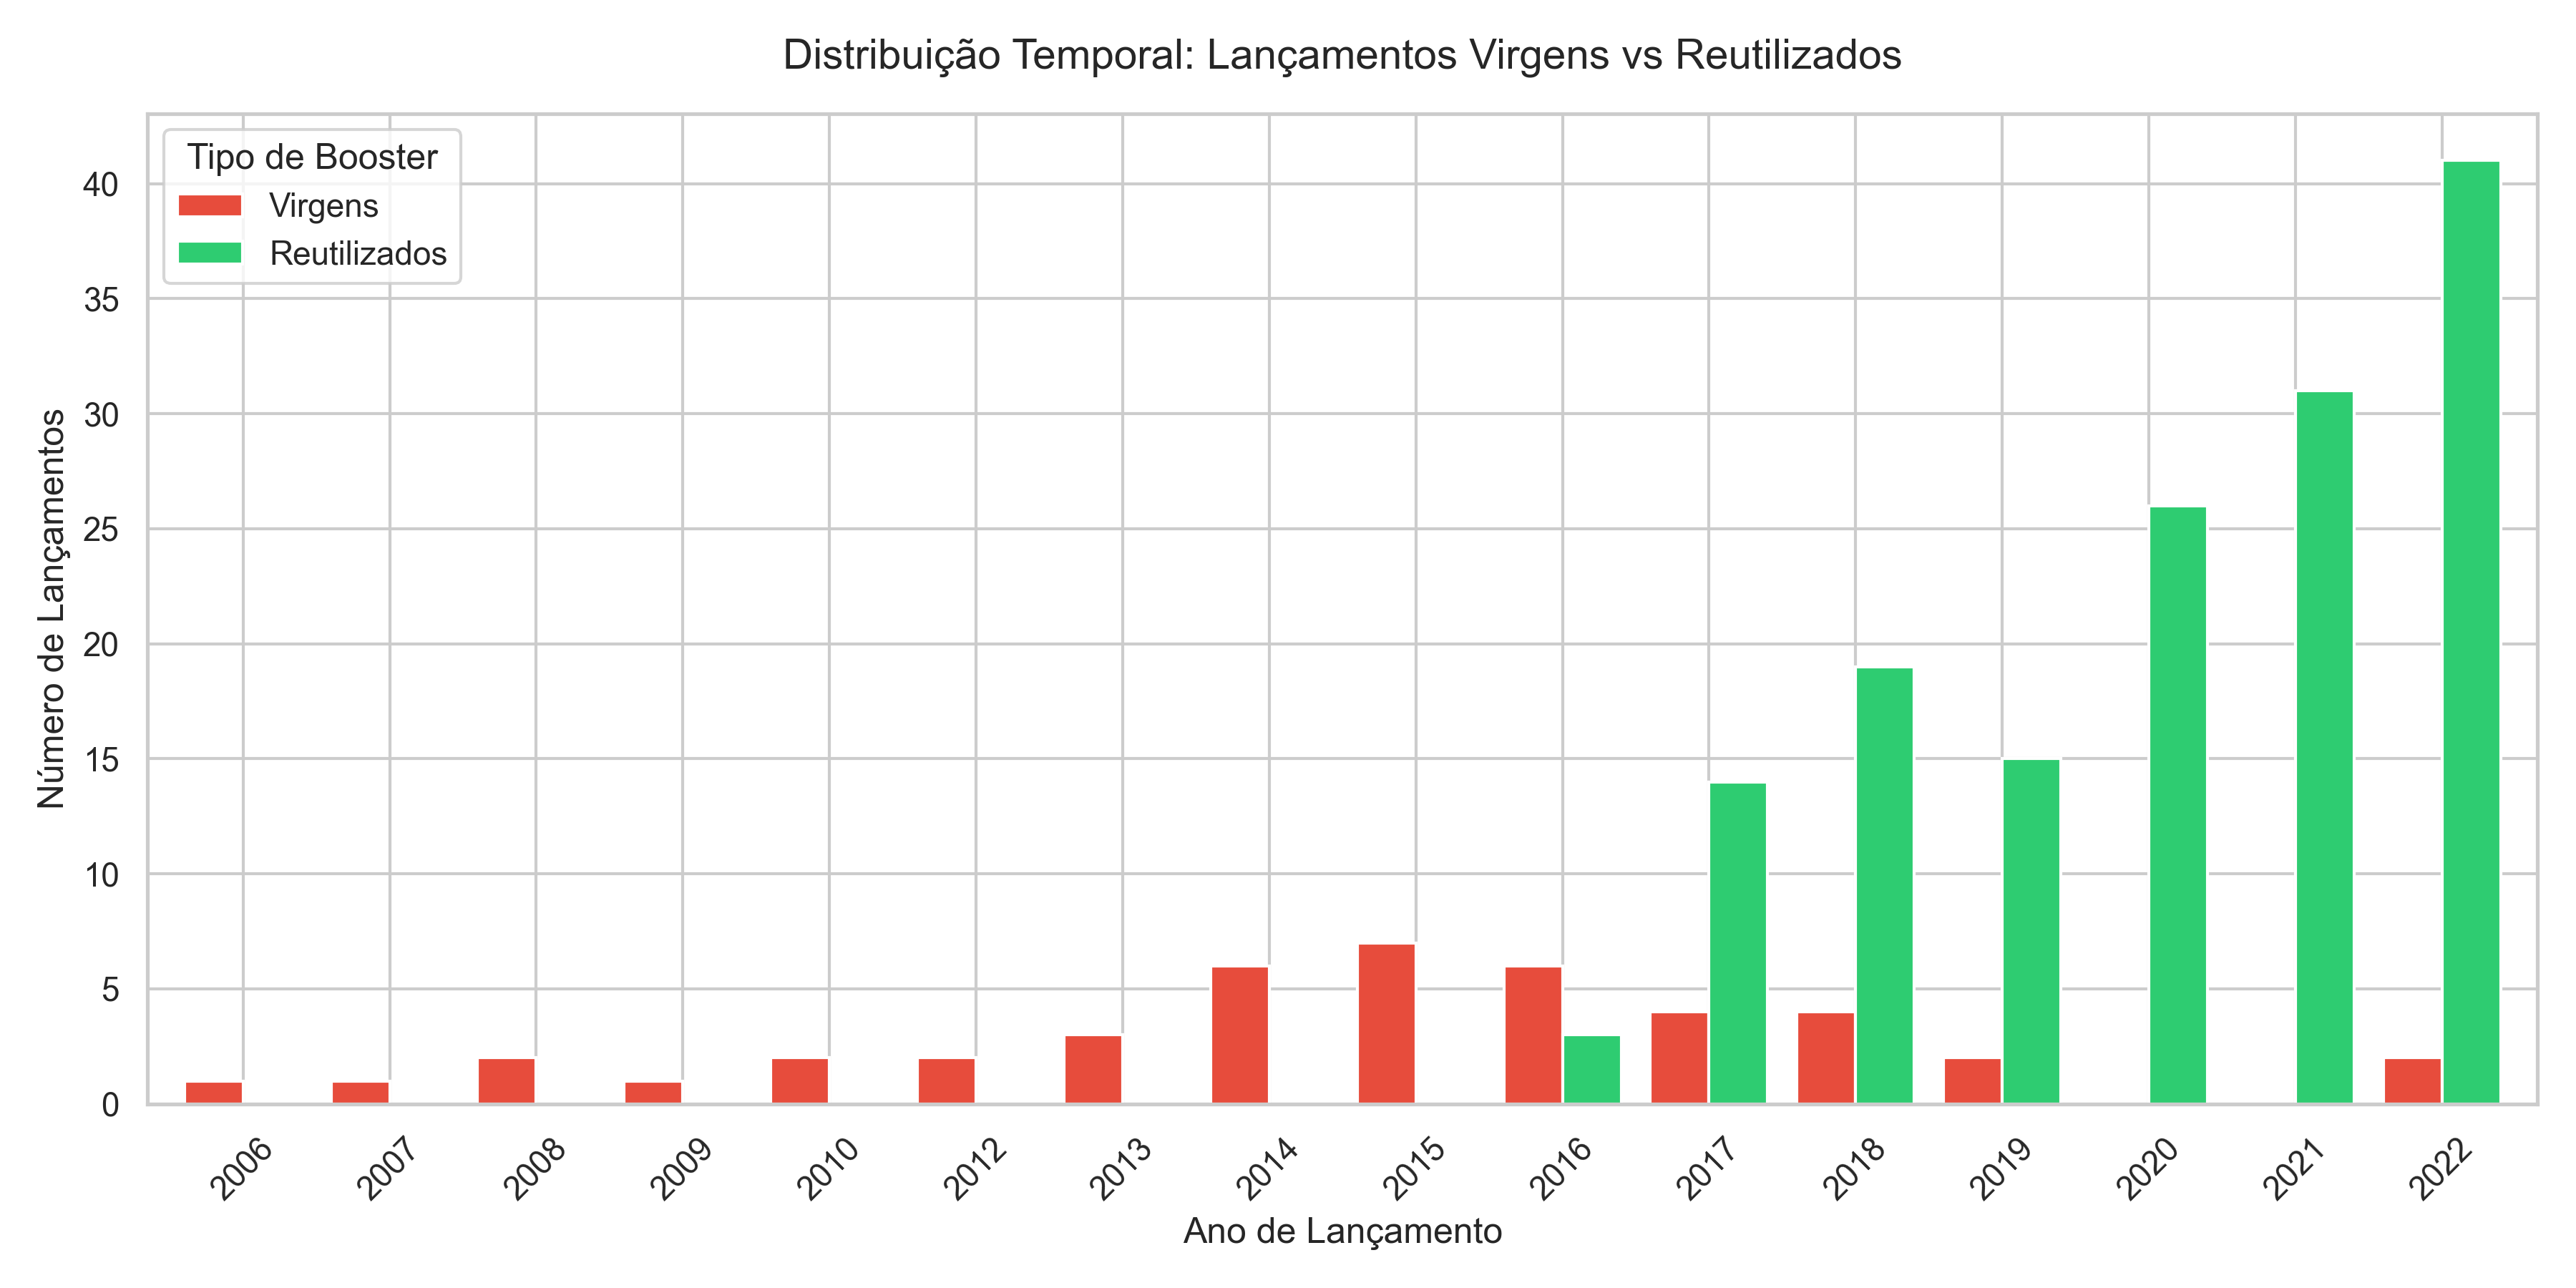
\includegraphics[width=0.85\textwidth]{kaio_temporal_distribution.png}
    \caption{Taxas de sucesso ao longo do tempo, separadas por tipo de booster.}
    \label{fig:kaio_temporal}
\end{figure}

% ══════════════════════════════════════════════════════════════════════════
\section{Experiência do Booster}
\label{sec:experience}

A análise de Izac aprofundou a investigação: em vez de apenas dividir entre ``virgem'' e ``reutilizado'', ele criou faixas de experiência para avaliar se existe algum padrão de degradação conforme o booster acumula mais voos.

\subsection{Estratificação por Faixas de Experiência}

Os resultados estão na \autoref{tab:izac_stats}. O padrão é bem claro: boosters em seu primeiro voo (novatos) têm taxa de sucesso de 88,37\%, mas a partir do segundo voo a taxa sobe para 100\% e se mantém em todas as faixas seguintes — independentemente de o booster ter 2 ou 13 voos anteriores.

\begin{table}[H]
\centering
\caption{Taxa de sucesso por faixa de experiência do booster.}
\label{tab:izac_stats}
\begin{tabular}{lrr}
\toprule
\textbf{Nível de Experiência} & \textbf{N} & \textbf{Taxa de Sucesso} \\
\midrule
Novatos (0 voos anteriores)       & 43  & 88,37\% \\
Intermediários (1--3 voos)        & 50  & 100,00\% \\
Experientes (4--6 voos)           & 30  & 100,00\% \\
Veteranos (7+ voos)               & 69  & 100,00\% \\
\bottomrule
\end{tabular}
\end{table}

\begin{figure}[H]
    \centering
    
\includegraphics[width=0.85\textwidth]{izac_experience_vs_success.png}
    \caption{Relação entre a experiência do booster e a taxa de sucesso.}
    \label{fig:izac_experience}
\end{figure}

\subsection{Ausência de Degradação}

Esse resultado é particularmente relevante: se houvesse desgaste acumulado nos boosters, seria de esperar que a taxa de sucesso caísse aos poucos com o aumento do número de voos. Mas não é isso que aparece nos dados. A relação se comporta mais como uma função degrau — o primeiro voo concentra todo o risco, e após esse ``batismo'', o booster mantém desempenho consistente.

% ══════════════════════════════════════════════════════════════════════════
\section{Famílias de Foguetes}
\label{sec:families}

Por fim, Jonatas comparou a confiabilidade das três famílias de foguetes operadas pela SpaceX.

\subsection{Comparação entre Famílias}

A \autoref{tab:jonatas_stats} mostra as taxas de sucesso de cada família. A diferença entre gerações é bastante visível: o Falcon 1 ficou em 40\%, o Falcon 9 em 98,9\% e o Falcon Heavy em 100\%.

\begin{table}[H]
\centering
\caption{Confiabilidade por família de foguete.}
\label{tab:jonatas_stats}
\begin{tabular}{lrrr}
\toprule
\textbf{Família} & \textbf{Total} & \textbf{Sucessos} & \textbf{Taxa de Sucesso} \\
\midrule
Falcon 1     & 5   & 2   & 40,0\% \\
Falcon 9     & 178 & 176 & 98,9\% \\
Falcon Heavy & 9   & 9   & 100,0\% \\
\bottomrule
\end{tabular}
\end{table}

\begin{figure}[H]
    \centering
    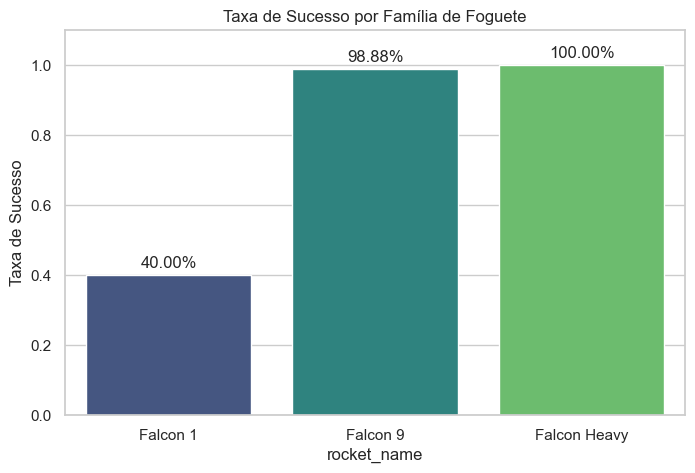
\includegraphics[width=0.85\textwidth]{jonatas_taxa_sucesso_familia.png}
    \caption{Taxa de sucesso por família de foguete.}
    \label{fig:jonatas_family}
\end{figure}

Do ponto de vista estatístico, o Falcon 9 é de longe o mais relevante pelo volume de dados disponível (178 registros). O Falcon Heavy tem resultado perfeito, mas com apenas 9 registros é difícil tirar conclusões fortes. Já o Falcon 1, operado entre 2006 e 2009, pertence a uma fase muito diferente da empresa — tanto em tecnologia quanto em experiência operacional.

%% sections/discussion.tex

\chapter{Discussão}
\label{chap:discussion}

Olhando para os resultados das quatro análises em conjunto, eles apontam numa mesma direção: não encontramos evidência de que a reutilização de boosters prejudique a confiabilidade das missões. Pelo contrário, os boosters reutilizados apresentaram desempenho superior aos virgens em todas as métricas que analisamos. Mas antes de aceitar essa conclusão, precisamos discutir os vieses e limitações que podem estar influenciando esses números.

\section{Visão Integrada}

A \autoref{tab:synthesis} resume o que cada análise encontrou.

\begin{table}[H]
\centering
\caption{Síntese dos resultados por eixo de análise.}
\label{tab:synthesis}
\begin{tabular}{p{3cm}p{5cm}p{4.5cm}}
\toprule
\textbf{Análise} & \textbf{Principal Achado} & \textbf{Confundidor} \\
\midrule
Temporal         & Sucesso evoluiu de 0\% para 100\% (2017--2022) & Mudança de família de foguete \\
Reutilização     & Reutilizados: 100\% vs.\ Virgens: 88,4\%      & Viés temporal + viés de seleção \\
Experiência      & Após 1º voo, 100\% em todas as faixas          & \textit{Survivorship bias} \\
Famílias         & F1: 40\% | F9: 98,9\% | FH: 100\%             & Tamanhos amostrais desiguais \\
\bottomrule
\end{tabular}
\end{table}

Quando juntamos as peças, a história que emerge é a seguinte: a análise temporal do Gabriel mostra que a SpaceX melhorou consistentemente ao longo do tempo, tanto em confiabilidade quanto em volume de operações. O Kaio mostrou que, nesse contexto, os boosters reutilizados nunca falharam. O Izac detalhou que o risco está concentrado no primeiro voo — depois disso, o booster mantém desempenho perfeito independentemente de quantas vezes voa. E o Jonatas mostrou que a evolução tecnológica entre as famílias de foguetes também teve papel importante nessa melhoria.

\section{Os Confundidores}

\subsection{Viés Temporal}

Esse é provavelmente o ponto mais delicado da nossa análise. A reutilização de boosters é um fenômeno recente — o primeiro booster reutilizado voou em 2016, época em que a SpaceX já tinha anos de experiência operacional com o Falcon 9. Então, quando dizemos que boosters reutilizados têm 100\% de sucesso, parte desse resultado pode simplesmente refletir o fato de que a empresa ficou melhor com o tempo, e não que a reutilização em si melhora a confiabilidade.

A análise temporal do Kaio ajuda um pouco a separar esses efeitos: nos anos em que os dois tipos de booster coexistem (2016--2022), os reutilizados continuam com desempenho perfeito. Mas mesmo assim, não dá para eliminar completamente essa dúvida com os dados que temos.

\subsection{Viés de Seleção}

Existe também um viés de seleção importante que não pode ser ignorado. Por definição, só são reutilizados os boosters que completaram pelo menos um voo com sucesso \textit{e} foram recuperados em boas condições. Ou seja, o grupo ``reutilizado'' já chega pré-filtrado — qualquer booster com defeito de fabricação ou problema estrutural tende a falhar no primeiro voo e ser descartado, nunca entrando na amostra de reutilizados.

A análise do Izac deixa isso especialmente claro: todos os boosters que ``sobrevivem'' ao primeiro voo mantêm 100\% de sucesso depois. Isso pode ser visto como uma confirmação de qualidade — mas também pode ser simplesmente o efeito de um filtro natural que elimina os boosters problemáticos antes que eles possam ser reutilizados.

\subsection{Tamanhos Amostrais}

As amostras dos diferentes grupos são bem desiguais. O Falcon 9 tem 178 registros, mas o Falcon 1 tem apenas 5 e o Falcon Heavy apenas 9. Da mesma forma, temos 149 boosters reutilizados contra 43 virgens. Essa assimetria limita a confiança que podemos ter nas comparações, especialmente para os grupos menores, cujos intervalos de confiança são bastante amplos.

\section{Outras Limitações}

Além dos confundidores que discutimos acima, vale mencionar algumas limitações adicionais:

\begin{itemize}
    \item A variável \texttt{success} só registra se o objetivo principal da missão foi atingido ou não. Problemas que não chegaram a comprometer a missão (como anomalias de pouso, por exemplo) não aparecem nos dados;

    \item O dataset vai apenas até 2022 e não inclui os lançamentos mais recentes, que envolvem boosters com números recordes de reutilização;

    \item Por ser um estudo observacional, não temos como atribuir causalidade — apenas associações. Seria necessário um experimento controlado para isso, o que obviamente não é viável nesse contexto;

    \item Todos os dados vêm de uma única fonte (SpaceX API mantida pela comunidade), o que pode introduzir imprecisões não documentadas.
\end{itemize}

%% sections/conclusion.tex

\chapter{Conclusão}
\label{chap:conclusion}

\section{Resposta à Pergunta de Pesquisa}

Voltando à pergunta que motivou este trabalho — \textit{a reutilização de foguetes afeta a confiabilidade das missões?} — a resposta, com base nos dados que analisamos, é que não encontramos evidência de impacto negativo.

Os números são, na verdade, favoráveis à reutilização: boosters que já haviam voado antes tiveram taxa de sucesso de 100\% em 149 registros, enquanto os boosters virgens ficaram em 88,37\% (38 de 43). Não identificamos nenhum sinal de degradação mesmo em boosters com até 13 voos acumulados, o que vai contra a intuição de que o uso repetido deveria desgastar os componentes e reduzir a confiabilidade.

A SpaceX, como empresa, melhorou muito ao longo do período analisado. A taxa de sucesso saiu de 0\% nos primeiros lançamentos em 2006 para 100\% sustentado a partir de 2017, ao mesmo tempo em que o volume de operações cresceu de forma significativa. Essa melhoria acompanhou tanto a evolução dos foguetes — do Falcon 1 ao Falcon 9 e ao Falcon Heavy — quanto a adoção cada vez maior da reutilização.

É importante, no entanto, não confundir correlação com causalidade. Os confundidores que identificamos (viés temporal, viés de seleção e tamanhos amostrais desiguais) são relevantes e impedem que afirmemos com certeza que a reutilização \textit{causa} mais confiabilidade. O que podemos afirmar é que, nos dados disponíveis, reutilizar boosters não prejudicou o desempenho das missões.

\section{Contribuições}

Este trabalho apresenta uma análise quantitativa dos lançamentos da SpaceX integrando quatro perspectivas complementares — temporal, reutilização, experiência do booster e famílias de foguetes. Além de responder à pergunta de pesquisa, o estudo identifica e documenta os principais confundidores que limitam a interpretação dos resultados, algo que frequentemente é negligenciado em análises mais superficiais sobre o tema.

\section{Trabalhos Futuros}

Algumas direções que podem ser exploradas em trabalhos futuros:

\begin{itemize}
    \item Atualizar o dataset com lançamentos mais recentes, especialmente os que envolvem boosters com mais de 20 voos;
    \item Aplicar métodos de inferência causal, como \textit{propensity score matching}, para tentar separar melhor o efeito da reutilização do efeito temporal;
    \item Incluir variáveis adicionais na análise, como massa da carga útil, tipo de órbita e local de lançamento;
    \item Ampliar a análise para outros operadores de lançamento (RocketLab, ULA) para contextualizar os resultados da SpaceX frente ao restante da indústria.
\end{itemize}


% ── Elementos pós-textuais ────────────────────────────────────────────────
\postextual

\bibliography{references}

\end{document}
